\chapter{Introduction}
\label{cha:intro}

Many machine-learning and deep-learning forecasters learn to predict an entity's future samples from its earlier observations. When the same entity supplies a long training history, the model can learn recurring temporal patterns together with characteristics specific to that entity. Testing that model on later dates measures how well it extrapolates the familiar series. By contrast, a newly observed entity must be forecast before a comparable training record exists.

A short local history reflects recent operating states but provides little evidence about seasonal cycles, extreme transitions, or plant-specific weather responses. The forecaster must therefore import cross-entity representations learned during pretraining or fleet adaptation and condition them on local context. Neither approach guarantees transfer: models often capture patterns specific to training installations that degrade when evaluated on an unfamiliar plant.

Figure~\ref{fig:problem_formulation} illustrates this knowledge transfer to unseen plants in the same region and in a new region.

\begin{figure}[H]
\centering
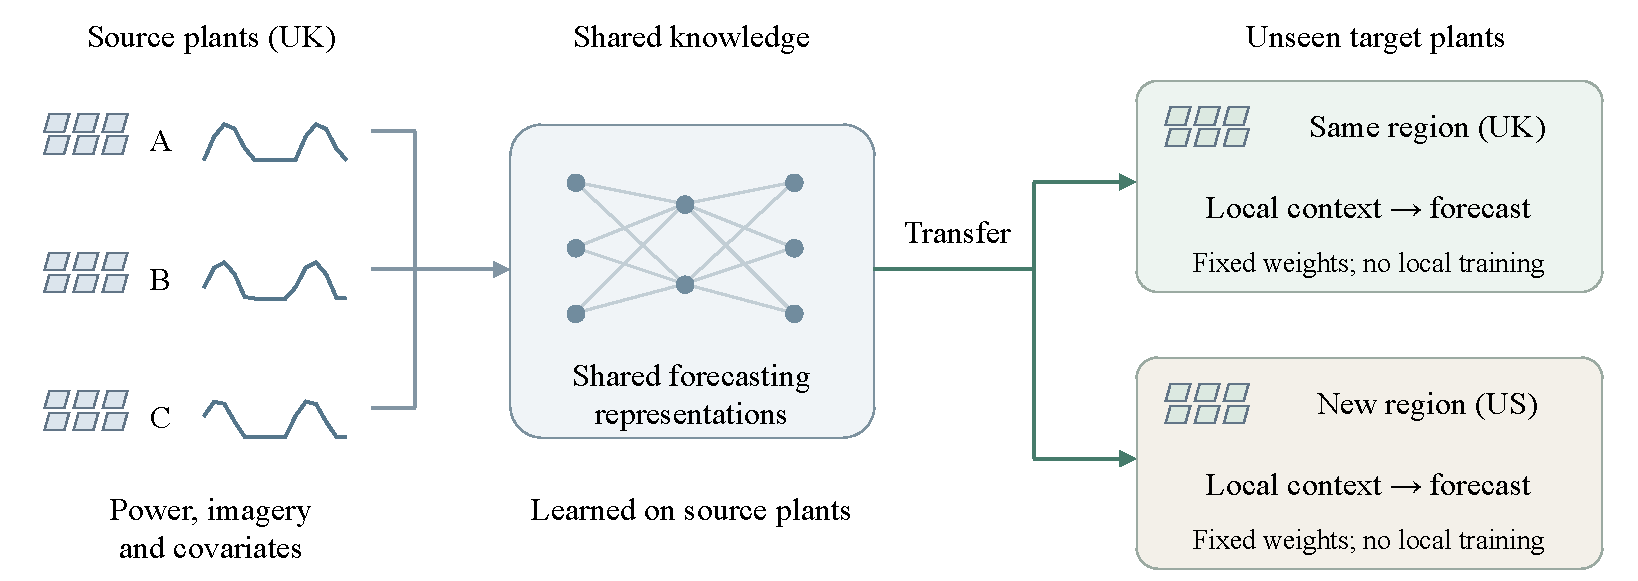
\includegraphics[width=0.95\textwidth]{figures/cross-plant-forecast-context.drawio.pdf}
\caption{Knowledge transfer to unseen plants in the same region and in a new region. Data from UK source plants adapt a shared forecaster. Its learned weights are then applied to held-out UK plants and to US plants without local training. In both settings, fourteen days of local power and environmental context condition a six-hour forecast. Target plants supply inputs but no weight updates. Traces and network symbols are schematic.}
\label{fig:problem_formulation}
\end{figure}

\newpage
Photovoltaic power makes the transfer problem concrete. The sun's position sets a regular daily pattern, but clouds can change output quickly, and the same conditions affect plants differently. Because these cloud-driven changes can occur within the six-hour forecast, recent power shows only what has already happened at the plant. Weather fields describe conditions over a wider area, while satellite images show the nearby cloud field. These sources differ in timing, spatial detail, and format, so the model must combine them for each forecast without a long training history from the target plant.

Figure~\ref{fig:pv_intermittency} compares clear conditions with a cloudy window containing repeated power ramps at held-out UK plant 11287. The clear-sky reference follows a smooth daily profile, but the cloudy-day measurements rise and fall sharply. Eight half-hour changes exceed ten percentage points of installed capacity, including a change larger than thirty percentage points. The satellite crops show the corresponding spatial observations.

\begin{figure}[H]
\centering
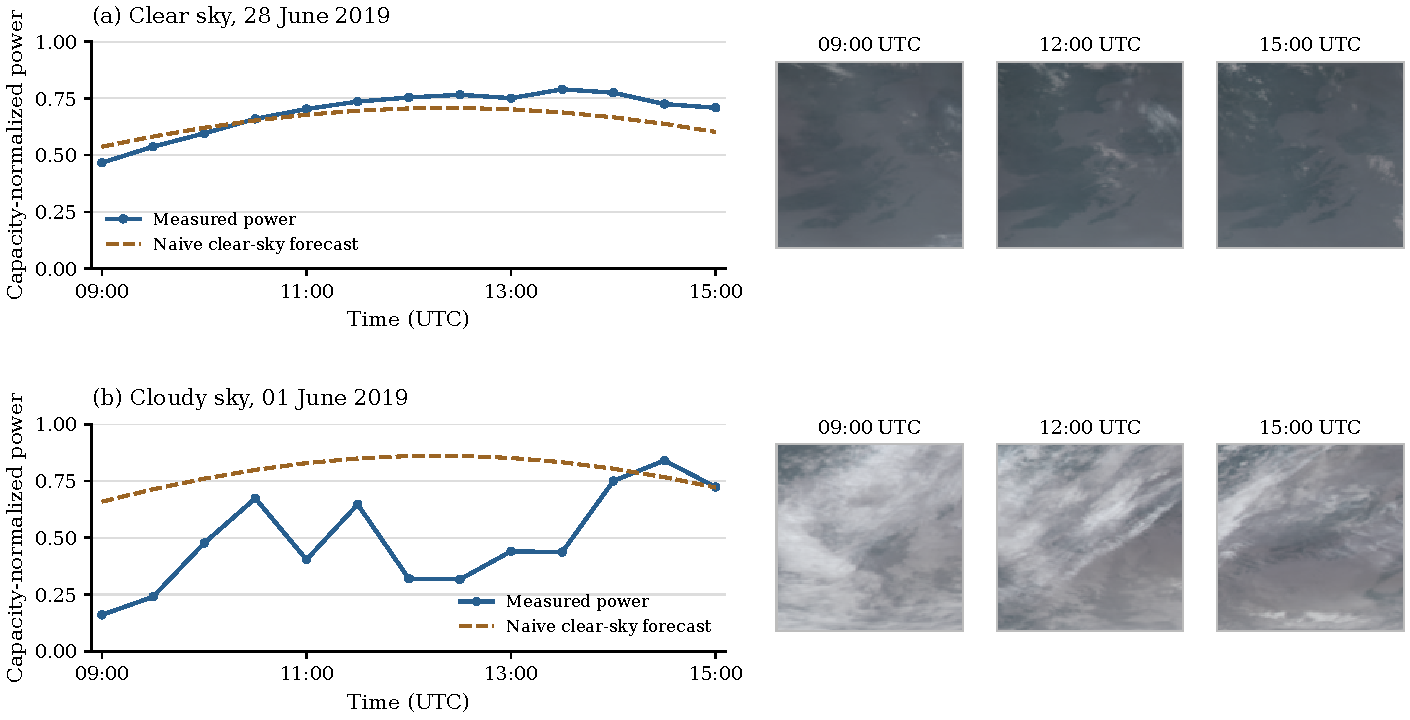
\includegraphics[width=0.98\textwidth]{figures/pv-power-satellite-context.pdf}
\caption{Clear-sky and cloudy conditions at UK plant 11287: (a) 28 June 2019; (b) 1 June 2019. Each row pairs a six-hour power trace with satellite observations of the same area. On the left, blue points show half-hourly measurements, joined by solid lines; a value of 0.5 denotes half the installed capacity. The orange dashed line is a naive clear-sky forecast, scaled using clear observations from the preceding fourteen days. The smooth profile in (a) contrasts with the repeated steep rises and falls in (b), which the reference forecast does not capture. On the right, display-enhanced infrared composites show cloud-field structure at 09:00, 12:00, and 15:00 UTC, read from left to right. The corpus is described in Chapter~\ref{cha:dataset}.}
\label{fig:pv_intermittency}
\end{figure}

This thesis studies that challenge by constructing an aligned numerical and satellite corpus, evaluating forecasts on plants excluded from fitting, and testing interfaces between a numerical foundation model and a frozen visual encoder.

\section{Forecasting from limited history and imagery}

Plants can differ in orientation, shading, local weather, and sensor behavior even after power is normalized by capacity. The forecaster must interpret a new plant's short record using patterns learned from other installations. The training, validation, and test sets therefore contain different plants. At each test forecast origin, the model receives fourteen days of recent power and permitted covariates. Models that use vision also receive satellite imagery. The model predicts the next six hours. The test plant supplies observations for that forecast, but no examples for fitting the model or its preprocessing statistics.

Satellite imagery may supply information that has not yet appeared in the plant's power trace. This visual context might help when a cloud system is approaching the array or when the local scene is represented more precisely than in the numerical covariates. The later controls examine these two explanations separately.

The challenge is to turn the visual field into a useful forecast input. A pretrained video encoder produces features over time and image location; the numerical foundation model processes patches of power and covariates. The thesis compares different interfaces while keeping the underlying numerical lineage and visual source as consistent as the experiments permit.

A higher multimodal benchmark score does not guarantee that the model actively uses the visual inputs. Structural modifications, regularizers, and optimization dynamics can alter predictions even when visual features contribute no useful signal. The evaluation protocol therefore couples benchmark scoring with zeroed-vision controls in fixed weights alongside temporal and spatial image substitutions to confirm whether the forecast genuinely relies on timely, site-matched imagery.

\section{Formal problem setting}

The task is a forecast for one plant from information available at a specified origin. The notation below defines the plant split, input window, target, and scoring rules; Chapter~\ref{cha:protocol} gives the experimental implementation.

\subsection{Plants, inputs, and forecast windows}

Plant identity and forecast time impose different constraints on a prediction. The split determines which installations can shape the fitted model, while the window determines what the model can observe when forecasting at a particular plant.

Let $i$ identify a plant and $t$ a forecast origin on its native power-sampling grid. Denote measured power at that time by $p_{i,t}$ and the plant's audited installed capacity by $c_i$. Capacity-normalized power is then $y_{i,t}=p_{i,t}/c_i$. At $t$, the model uses recent normalized power and numerical covariates describing atmospheric conditions, solar geometry, and calendar time. Multimodal methods also use a recent satellite clip when imagery is available.

Let $\mathcal{P}$ denote the complete set of plants, with $\mathcal{P}_{\mathrm{train}}$, $\mathcal{P}_{\mathrm{val}}$, and $\mathcal{P}_{\mathrm{test}}$ denoting the training, validation, and test subsets. These subsets are pairwise disjoint and cover all plants:

\[
\mathcal{P} = \mathcal{P}_{\mathrm{train}} \cup \mathcal{P}_{\mathrm{val}} \cup \mathcal{P}_{\mathrm{test}},
\]

In particular,

\[
\mathcal{P}_{\mathrm{train}} \cap \mathcal{P}_{\mathrm{test}} = \emptyset
\]

and the same condition holds for validation against the other two subsets. Model weights, preprocessing statistics, and retrieval stores are fitted without test-plant examples; Chapter~\ref{cha:protocol} specifies the safeguards.

Let $H$ be the number of past power samples, $h$ the number of future power samples, and $L$ the number of satellite frames in a window. The physical history and forecast durations determine $H$ and $h$ at the plant's cadence; $L$ follows the image cadence. Let $x$ denote permitted numerical covariates, $v$ satellite frames, and $m$ validity masks. For plant $i$ at origin $t$, the window operator $\mathcal{W}(i,t)$ pairs the inputs with the future-power target:

\[
\mathcal{W}(i,t) = \left(y_{i,t-H+1:t}, x_{i,t-H+1:t+h}, v_{i,t-L+1:t}, m_{i,t-H+1:t+h}, y_{i,t+1:t+h}\right).
\]

The first component is the power history through $t$; the final component is the target from the following $h$ steps and is withheld from the model. The covariate and mask components cover the indicated history and forecast intervals.

The slice of $v$ is shorthand for the $L$ frames selected by UTC time up to the origin; its indices do not imply that images share the power-sampling grid. Keeping the two clocks separate avoids discarding frames or inventing intermediate ones. Chapter~\ref{cha:method} specifies the visual encoder's latent shapes and token selection.

\subsection{Predictions and scoring}
\label{sec:metric-definitions}

For each window, the forecaster predicts quantiles of future capacity-normalized power, following the direct quantile-regression formulation of Chronos-2~\cite{chronos2}. This study uses nine levels from 0.1 to 0.9. Pinball loss is suited to these outputs because it weights underprediction by the quantile level and overprediction by its complement. Minimizing the loss at a given level therefore estimates that conditional quantile. For level $\tau\in(0,1)$, target $y$, and prediction $\hat{y}^{\tau}$, the loss is

\[
\rho_{\tau}(y-\hat{y}^{\tau}) =
\begin{cases}
\tau(y-\hat{y}^{\tau}) & \text{if } y \geq \hat{y}^{\tau},\\
(1-\tau)(\hat{y}^{\tau}-y) & \text{otherwise}.
\end{cases}
\]

Let $\mathcal{Q}$ be the set of nine quantile levels, $b$ index windows in a batch, and $k$ index forecast steps. The target mask $m_{b,k}$ is one for a valid target and zero otherwise. The training objective combines the pinball losses over these indices:

\[
\mathcal{L}_{\mathrm{pin}} = \frac{\sum_{b,k,\tau} m_{b,k}\rho_{\tau}(y_{b,k}-\hat{y}_{b,k}^{\tau})}{\sum_{b,k} m_{b,k}\,|\mathcal{Q}|}.
\]

As in Chronos-2, unavailable targets contribute no loss. Dividing by the number of valid targets and quantile levels keeps the objective's scale from changing merely because a batch has more missing values. Replacing a missing target by zero would instead teach the model that a logging gap is a night-time observation.

The median quantile supplies the point forecast, denoted $\hat{y}$, used by normalized mean absolute error (NMAE) and normalized root mean squared error (NRMSE). The outer quantiles define prediction intervals, while the complete quantile set supports the continuous ranked probability score (CRPS) and calibration analysis. Forecasting the horizon in one pass avoids feeding an earlier prediction back as input to a later step.

For a set of valid forecast points $\mathcal{S}$, normalized mean absolute error and normalized root mean squared error are

\[
\mathrm{NMAE} = \frac{1}{|\mathcal{S}|}\sum_{(i,t)\in\mathcal{S}} |y_{i,t}-\hat{y}_{i,t}|,
\]

\[
\mathrm{NRMSE} = \sqrt{\frac{1}{|\mathcal{S}|}\sum_{(i,t)\in\mathcal{S}} (y_{i,t}-\hat{y}_{i,t})^2}.
\]

Because $y$ is already capacity normalized, both quantities are dimensionless. Chapter~\ref{cha:protocol} specifies plant weighting, valid-step masking, and the ramp subset used for the co-primary comparison.

Skill score is commonly used in PV forecasting to express improvement over a reference method~\cite{singh2026pvforecastreview}. Here Smart Persistence is the reference, so the score shows how much NRMSE the model removes beyond a simple forecast evaluated on the same targets:

\[
\mathrm{SS} = 100\left(1-\frac{\mathrm{NRMSE}_{\mathrm{model}}}{\mathrm{NRMSE}_{\mathrm{SP}}}\right).
\]

A score of zero matches Smart Persistence; positive values improve on it, and negative values perform worse. The subscript SP identifies that reference forecast. The factor of 100 makes a value of 55.10 a 55.10 percent reduction in NRMSE.

Ramp NMAE evaluates forecast error during rapid swings in power output. Rapid changes challenge grid operators because steep ramps require fast-acting reserve power. For each plant $i$, the evaluator computes the absolute change between consecutive valid readings, $\Delta_{i,t} = |y_{i,t} - y_{i,t-1}|$, using the final history step for the first forecast lead. The ramp subset $\mathcal{S}_{\mathrm{ramp}} \subset \mathcal{S}$ contains the valid daylight target steps where $\Delta_{i,t}$ meets or exceeds the plant's 90th percentile threshold $\gamma_i$, selecting the top decile of observed changes across the test set. Ramp NMAE is then calculated as the mean absolute error over these ramp instances:

\[
\mathrm{Ramp\ NMAE} = \frac{1}{|\mathcal{S}_{\mathrm{ramp}}|}\sum_{(i,t)\in\mathcal{S}_{\mathrm{ramp}}} |y_{i,t}-\hat{y}_{i,t}|.
\]

Because the ramp subset is derived entirely from observed power, all models are evaluated on the exact same timestamps regardless of their predicted values.

The nine quantiles also allow forecast uncertainty to be assessed within the framework of strictly proper scoring rules~\cite{gneiting}. The continuous ranked probability score (CRPS) approximation combines their pinball losses into one score, equal to twice the mean loss across quantile levels, where lower values indicate superior performance. Interval coverage at nominal level $\alpha$ is the fraction of observed targets that fall between the corresponding lower and upper quantiles. At each quantile level, the gap is between its stated probability and the fraction of targets that actually fall below it. Quantile expected calibration error averages these gaps across levels.

\section{Research questions}

Under the plant-disjoint split and scoring rules above, the central question is whether combining a time-series foundation model with a visual foundation model improves six-hour forecasts at unseen plants. The visual arms are fitted on other UK plants but receive no fitting on test plants. The numerical comparison tests whether adapting the backbone on training plants improves on that baseline. The visual comparisons ask whether recent, plant-aligned imagery adds information beyond power history and permitted covariates, and whether the fusion interface affects how much of that information reaches the forecast. In addition, the benchmark evaluates retrieval mechanisms and parameter-efficient adapters as non-visual baselines to assess how much transfer can be achieved without image processing.

An inference-only evaluation then applies the UK-trained models to eight US plants across three matched training seeds. It tests whether the within-UK ranking and visual contribution persist when both region and satellite source change. 

\section{Contributions}

The thesis makes three contributions:

\begin{enumerate}
\item \textbf{Corpus.} It aligns plant power, numerical context, and satellite imagery across UK and US tracks while retaining sample-level provenance.
\item \textbf{Benchmark.} It defines a plant-disjoint evaluation under explicit input and scoring rules. The benchmark compares reference forecasts, supervised models, time-series foundation models, retrieval and adaptation methods, and multimodal systems.
\item \textbf{Fusion analysis.} It compares pooled and spatially addressable visual interfaces. Same-weights and content-substitution controls show reliance on recent, site-specific imagery.
\end{enumerate}

\section{Scope and wider relevance}

Photovoltaic power is the testbed for a broader transfer problem: forecasting for an entity absent from training using a short local history and a spatial observation of its environment. A newly commissioned wind farm presents a similar combination of turbine records and approaching weather. An ungauged basin can pair a short streamflow record with satellite observations of upstream conditions. New fields, monitored districts, substations, and traffic links may also have thin local histories and spatial context. These examples share the information structure; the thesis does not measure transfer to those domains.

The scope of this thesis centers on solar power generation forecasting. Upstream surface irradiance modeling and downstream grid applications, including market bidding, economic dispatch, and inverter control, remain outside the empirical evaluation.

\section{Thesis structure}

Chapter~\ref{cha:related} situates the cross-plant transfer problem within statistical, deep sequence, and foundation-model literature. Chapter~\ref{cha:dataset} details the multimodal corpus across the UK and US tracks, and Chapter~\ref{cha:method} introduces the MMTSFM fusion ladder. Chapter~\ref{cha:protocol} formalizes the plant-disjoint evaluation protocol and diagnostic interventions. Chapters~\ref{cha:results} and~\ref{cha:ablations} report benchmark rankings and ablation findings, followed by a discussion of visual reliance in Chapter~\ref{cha:discussion} and concluding directions in Chapter~\ref{cha:conclusions}.
